\section{Expressões Gerais para os Coeficientes de $\mathbf{A_{II}}$ e $\mathbf{A}_{FF}$}

Resolvendo os sistemas de equações algébricas~\ref{eq:caso1-Aii} e~\ref{eq:caso2-Aff}, cuja ordem é o número de graus de liberdade por elemento, podem-se avaliar as quantidades de interesse para formulações do Método dos Deslocamentos.

A partir da relação~\ref{eq:Aii}, as fórmulas explícitas para calcular os coeficientes são determinadas de acordo com os dois casos mostrados na figura~\ref{fig:casos-considerados}. Tem-se:

\subsection*{Caso I: O nó final é engastado}
Neste caso, as expressões dos esforços internos M, N e Q, causados por ações $f_{kj}$ e $\bar{f}_i=1,k,j=1,2,3$, são determinadas por (veja Fig.~\ref{fig:rep-el-eixo-local})

\begin{align}
	M_{1j} = Q_{1j} = 0, \quad
	N_{1j} = -f_{1j},\nonumber & \\
	M_{2j} = f_{2j}x'_1, \quad
	Q_{2j} = f_{2j}, \quad
	N_{2j} = 0, \nonumber      & \\
	M_{3j} = -f_{3j}, \quad
	Q_{3j}=N_{3j}=0.
	\label{eq:esforcos-internos1}
\end{align}

e, as expressões correspondentes para $\bar{M}_i$, $ \bar{N}_i$ e $\bar{Q}_i, \; i=1,2,3$, são obtidas através das expressões dadas em~\ref{eq:esforcos-internos1} com $f_i=\bar{f}_i=1$,i.e.,
\begin{align}
	\bar{M}_1=\bar{Q}_1 = 0, \quad
	\bar{N}_1 = -1 \nonumber & \\
	\bar{M}_2 = x'_1, \quad
	\bar{Q}_2 = +1, \quad
	\bar{N}_2 = 0, \nonumber & \\
	\bar{M}_3 = -1, \quad
	\bar{Q}_3=0, \quad
	\bar{N}_3=0.
\end{align}

\begin{figure}[!htbp]
	\centering
	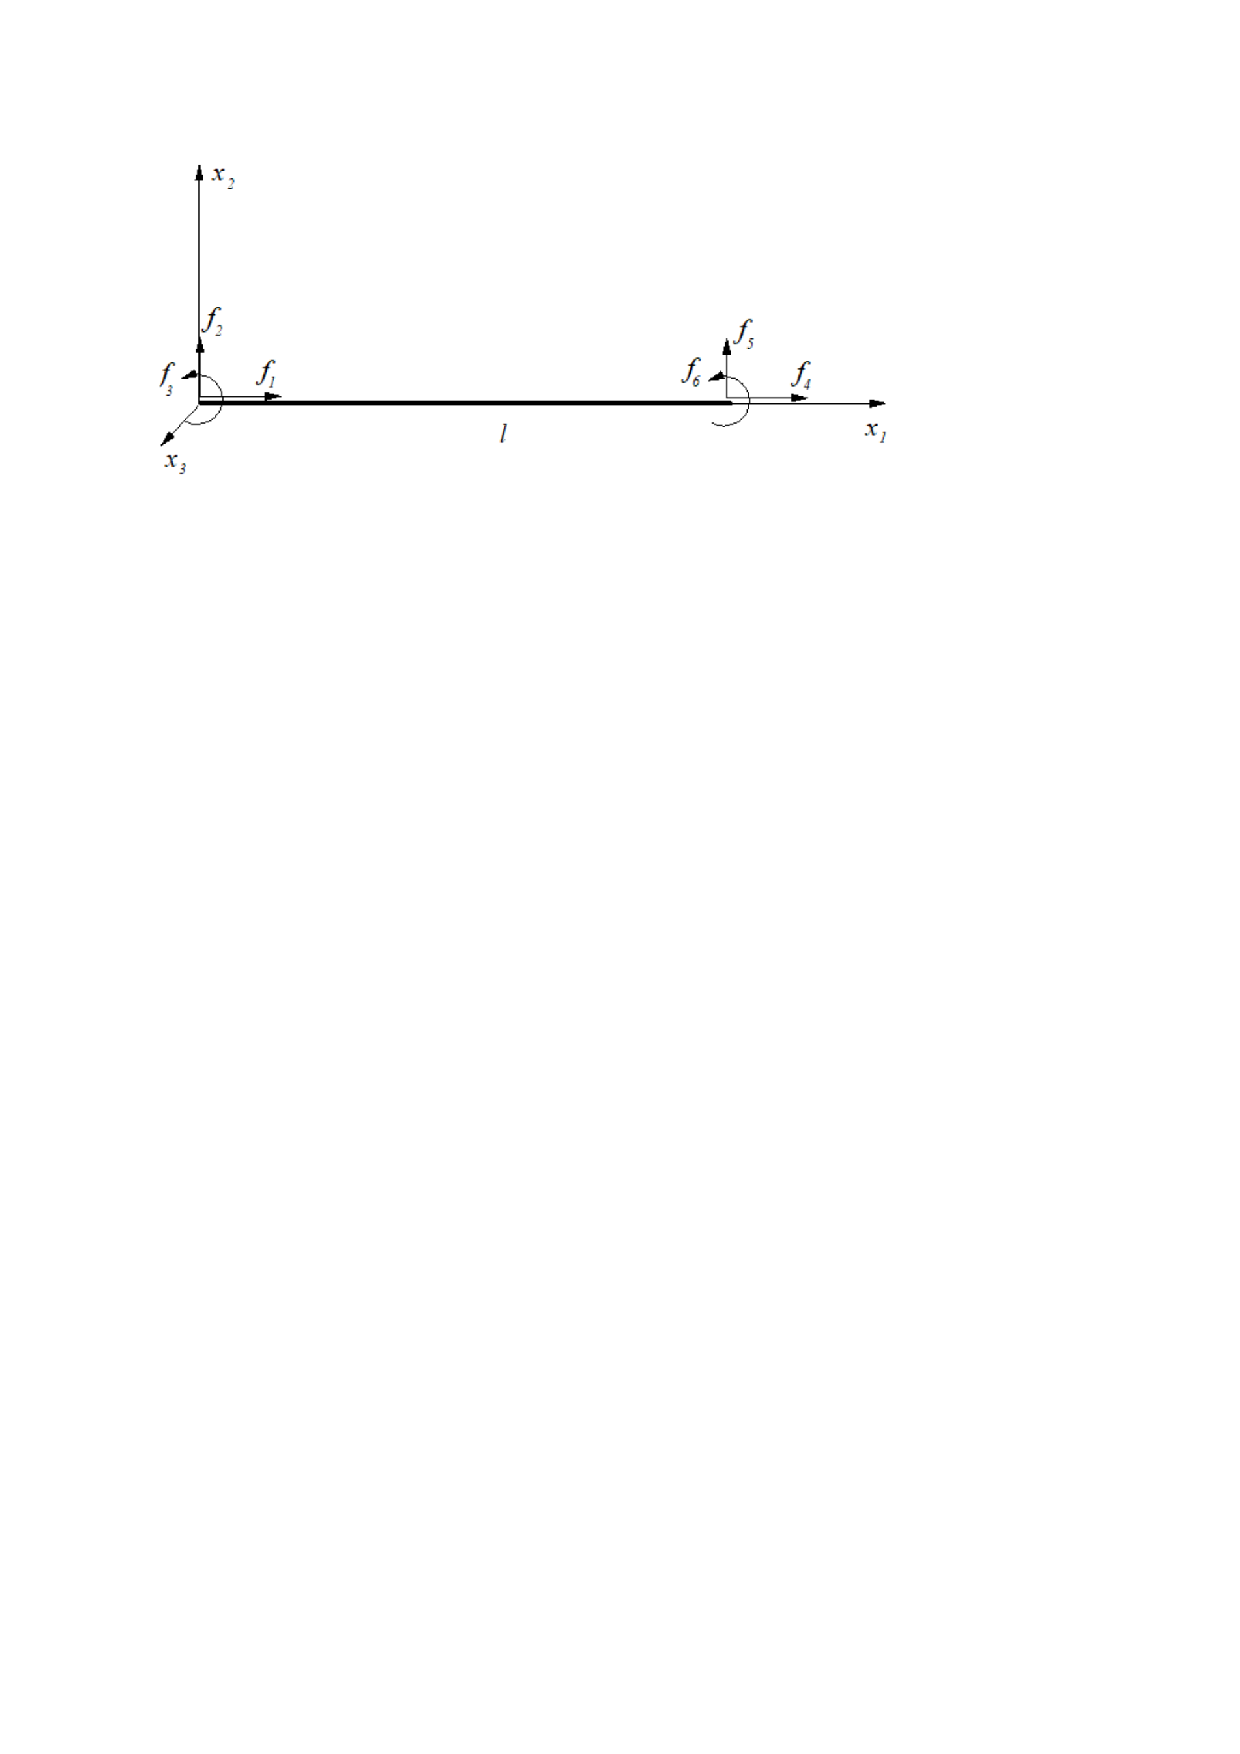
\includegraphics[trim = 10mm 220mm 45mm 25mm, clip, scale=1]{img/rep-el-eixo-local}
	\caption{Representação do elemento no eixo local $x'_1, x'_2$ e $x'_3$.}
	\label{fig:rep-el-eixo-local}
\end{figure}

Resulta, finalmente:
\begin{equation*}
	\label{eq:coeficientes_Aii}
	\begin{array}{ccc}
		a_{11} = \int_l \dfrac{1}{k_a}\,dx'_1, & a_{12} = 0,                                                                & a_{13} = 0,                                \\
		a_{21} = 0,                            & a_{22} = \int_l \left( \dfrac{x_1^2}{k_b} + \dfrac{1}{k_s} \right)\,dx'_1, & a_{23} = -\int_l \dfrac{x_1}{k_b} \,dx'_1, \\
		a_{31} = 0,                            & a_{32} = -\int_l \dfrac{x_1}{k_b} \,dx'_1,                                 & a_{33} = \int_l \dfrac{1}{k_b}\,dx'_1.
	\end{array}
\end{equation*}

\subsection*{Caso II: O nó inicial é engastado}

As expressões para M, N e Q, causados por ações $f_{kj}$, $k,j=4,5,6$, são
\begin{align}
	\label{eq:esforcos-internos2}
	M_{4j} = Q_{4j} = 0, \quad
	N_{4j} = f_{4j}, \nonumber & \\
	M_{5j} = f_{5j}(l-x'_1), \quad
	Q_{5j} = -f_{5j}, \quad
	N_{5j} = 0, \nonumber      & \\
	M_{6j} = f_{6j}, \quad
	Q_{6j}=N_{6j}=0.
\end{align}

e, as funções correspondentes $\bar{M}_i$, $\bar{N}_i$ e $\bar{Q}_i$, causadas por $\bar{f}_i=1,i=4,5,6$ são obtidas pelas expressões~\ref{eq:esforcos-internos2} substituindo-se $f_{kj}$ por $\bar{f}_i$.

\begin{align}
	\bar{M}_4=\bar{Q}_4 = 0, \qquad
	\bar{N}_4 = +1 \nonumber & \\
	\bar{M}_5 = (l-x'_1), \qquad
	\bar{Q}_5 = -1, \qquad
	\bar{N}_5 = 0  \nonumber & \\
	\bar{M}_6 = +1, \qquad
	\bar{Q}_6=0,  \qquad
	\bar{N}_6=0.
\end{align}

Assim, obtém-se, da relação~\ref{eq:Aii}:

\begin{equation}
	\label{eq:coeficientes_Aff}
	\begin{array}{ccc}
		a_{44} = \int_l \dfrac{1}{k_a}\,dx'_1, & a_{45} = 0,                                                                    & a_{46} = 0, \nonumber                                   \\
		a_{54} = 0,                            & a_{55} = \int_l \left( \dfrac{(l-x_1)^2}{k_b} + \dfrac{1}{k_s} \right)\,dx'_1, & a_{56} = \int_l \dfrac{(l-x_1)}{k_b} \,dx'_1, \nonumber \\
		a_{64} = 0,                            & a_{65} = \int_l \dfrac{(l-x_1)}{k_b} \,dx'_1,                                  & a_{66} = \int_l \dfrac{1}{k_b}\,dx'_1.
	\end{array}
\end{equation}

A avaliação das integrais nas equações~\ref{eq:coeficientes_Aii} e~\ref{eq:coeficientes_Aff}, exceto para elementos física e geometricamente uniformes, não pode ser feita analiticamente. Em casos gerais de variação de rigidez $k_b$ e $k_s$ um esquema de integração numérica deve ser empregado. Neste projeto foi utilizado o processo de integração de Gauss-Legendre. Assim, após obtidas as expressões gerais para os coeficientes $a_{ij}$, dadas acima, resulta:

\begin{equation}
	\label{eq:gauss-legendre}
	a_{ij} = \int_l g_{ij}(x'_1)\,dx'_1 = \dfrac{l}{2}\sum_{k=1}^{\textrm{npg}} g_{ij}[x'_1(\eta_k)]\omega_k,
\end{equation}

onde o integrando relaciona-se com o coeficiente $a_{ij}$ a ser calculado, $\eta_k$ é a abscissa do k-ésimo ponto de integração, $\omega_k$ é fator de pesagem correspondente, e npg é o número de pontos de integração usado (usualmente considera-se $\textrm{npg} \leq 4$).

Com o procedimento proposto neste artigo, podem-se obter as seguintes expressões genéricas para os coeficientes de rigidez e ações de engastamento:
